\chapter{Psalm 66}

\begin{figure}
  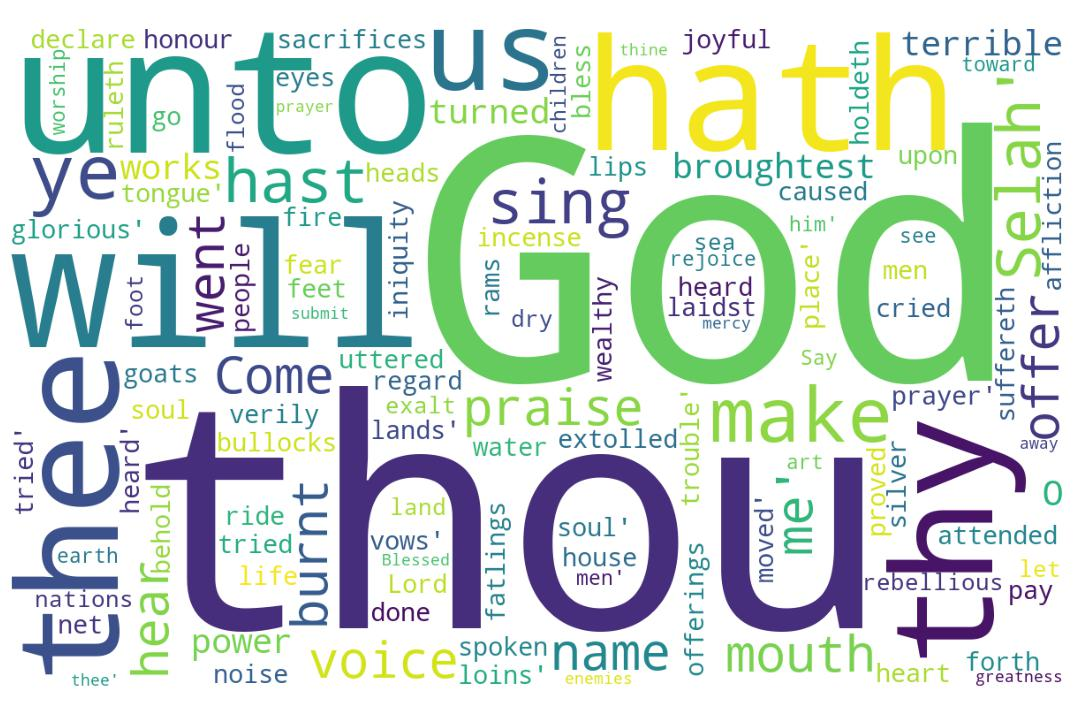
\includegraphics[width=\linewidth]{19OT-Psalms/Psalm66-WordCloud.jpg}
  \caption{Psalm 66 Word Cloud}
  \label{fig:Psalm 66 word Cloud}
\end{figure}

\marginpar{\scriptsize \centering \fcolorbox{bone}{lime}{\textbf{BE THANKFUL}}\\ (Psalm 66:1-20) \begin{compactenum}[I.][8]
    \item The \textbf{Prime Directive} (Futility) \index[scripture]{Psalms!Psa 066:01} Psa 66:1
    \item The \textbf{Path that was Dry}  \index[scripture]{Psalms!Psa 066:06} Psa 66:6
    \item \textbf{Perpetual Dominion} \index[scripture]{Psalms!Psa 066:07} Psa 66:7
    \item A \textbf{Profitable Decision} \index[scripture]{Psalms!Psa 066:13} Psa 66:13
    \item A \textbf{Positive Declaration} \index[scripture]{Psalms!Psa 066:16} Psa 66:16
    \item A \textbf{Pure Difference} \index[scripture]{Psalms!Psa 066:18} Psa 66:18
\end{compactenum}}

\footnote{\textcolor[rgb]{0.00,0.25,0.00}{\hyperlink{TOC}{Return to end of Table of Contents.}}}\footnote{\href{https://audiobible.com/bible/psalms_66.html}{\textcolor[cmyk]{0.99998,1,0,0}{Psalm 66 Audio}}}\textcolor[cmyk]{0.99998,1,0,0}{To the chief Musician, A Song \emph{or} Psalm.}\\
\\
\P \textcolor[cmyk]{0.99998,1,0,0}{Make a \fcolorbox{bone}{lime}{joyful noise} unto God, all ye lands:} %\footnote{Most of this Psalm deals with the Second Advent. Verses 3, 7, 12--13, and 15 are all Millennial references, and the Jews’ “tribulations” will be found in verses 10---12, and 14. You may expect the usual. The “godly” commentators will either miss the doctrinal import of the verses completely or, like Jamieson and Kroll, they will “hint” that perhaps the verses have a future application to some victory, by someone over someone, that will eventually take place sometime. Muddled incoherence is one the characteristics of the exegesis by apostate Fundamentalists when they hit a verse in the King James English that they either don’t like or cannot understand. (This is amply demonstrated in our Commentary on the Psalms). “All ye lands” (vs. 1). This means the heathen (the Gentiles), as in Deuteronomy 32:43 and Romans 11:12--13. Of course, we can make spiritual application. A “joyful noise” by a congregation is better than a smooth, slick, well-executed choir number by professional TV watchers (see Ps. 33:3). The Gregorian chants and Latin “masses” and “requiems” are exactly what is NOT meant by the verse. The song is aimed at God, not the listener (“unto God”). His honor is to be sung, and His praise is to be made “glorious.” The text of the song is given, for the wording follows “Say unto God.” The crucial “Selah” pops up again (for the fortieth time) to warn the “qualified authorities” and “recognized scholars” they are in trouble if they don’t believe THE BOOK. \\
%\\
%Good old Kroll (representing Liberty University) slides by as smooth and slick as a garter snake in a pool of oil. He puts verse 1 in the present tense to get rid of Deuteronomy 32:43 and Isaiah 14:7, and then expostulates on verse 4 saying, “His enemies shall be brought to forced submission under His feet.” Who are His enemies? Zero. When are they brought into submission? Zero. Is “under His feet” literal (Isa. 63:1--6) or figurative? Zero. This is the Swindoll-MacArthur-Bob Jones IV “life-style.” Get through without being detected. Don’t let ’em know what you believe. It is too costly. Dummelow and Kyle Yates are much more honest: one throws the verse out, and the other one says, “The Psalmist takes the whole world in at one sweep, as he sounds the call and gives the proper words for the expression of true praise,” which, of course, means absolutely NOTHING. If we accepted Kroll’s sterile and ambiguous comments, think what we would be missing, even devotionally. 1. Where are the joyful songs about the names of Mohammed, Buddha, Mao Tsetung, Brahma, the popes, and Moses? It says “sing to thy name” (vs. 4). Singing is a manifestation of JOY (“make a joyful noise”). Where are ten songs praising Buddha? Where are fifty praising Mohammed? I have four different hymn books in my house, and between them they present seven hundred different songs about one man. My two German hymnals have fifty more songs which are not in the English hymnals. How does the founder of one religion rate seven hundred fifty songs, while all the others combined can’t produce two hundred songs? Someone’s religion fails to produce JOY. 2. “Thy name” is recommended, so out come Jesus Saves, What a Friend We Have in Jesus, My Jesus I Love Thee, Fairest Lord Jesus, Jesus Is The Sweetest Name I Know, No One Ever Cared for Me Like Jesus, The Light of the World Is Jesus, Jesus What a Friend of Sinners, Jesus the Very Thought of Thee, etc.\cite{Ruckman1992Psalms} }
[2] \textcolor[cmyk]{0.99998,1,0,0}{Sing forth the honour of his name: make his praise glorious.}
[3] \textcolor[cmyk]{0.99998,1,0,0}{Say unto God, How terrible \emph{art} \emph{thou} \emph{in} thy works! through the greatness of thy power shall thine enemies submit themselves unto thee.} %\footnote{The song of verses 2 and 3 has at times come to your ears; for, as Talmage says: “I think sometimes it must break out over the battlements of heaven where the hosts are engaged in perpetual praise.” It is a song about “JESUS”—the One who made our solar system, the One who gave us life, the One who protected us as children, the One who brought us through many dangers, toils, and snares, the One who redeemed us and granted us the New Birth, and the One who will meet us at the end of the race (Hebrews 12:1--3), and grant us an eternity of enjoying the presence of God.\cite{Ruckman1992Psalms} }
[4] \textcolor[cmyk]{0.99998,1,0,0}{All the earth shall worship thee, and shall sing unto thee; they shall sing \emph{to} thy name. Selah.}
[5] \textcolor[cmyk]{0.99998,1,0,0}{Come and see the works of God: \emph{he} \emph{is} terrible \emph{in} \emph{his} doing toward the children of men.} %\footnote{The word “terrible,” verse 5, is used in the sense of “awesome” (as in verse 3), not as the word “rotten” is used today. Observe the same thing in Revelation 17:6 where the word “admiration” is used in the sense of “awesome,” not in the sense of something to be worshipped or bragged about. \cite{Ruckman1992Psalms} }
[6] \textcolor[cmyk]{0.99998,1,0,0}{He turned the sea into \fcolorbox{bone}{lime}{dry \emph{land}}: they went through the flood on foot: there did we rejoice in him.} %\footnote{Verse 6, historically, is the Red Sea crossing. All of the commentators (100 percent) missed the advanced revelation given 380 years ago, that it will happen again in Revelation 12:15, which matches the “flood” prophesied in Daniel 9:26. This flood is connected with the Jordan River (Job 40:23). Note that the first song --  and the context of verse 6 is singing (vss. 1--2) -- was sung at the Red Sea crossing (Exod. 15:1). The “song of Moses” is sung by the Tribulation Saints (Rev. 15:3): “there did we rejoice in him” (vs. 6). The “water” of verse 12 that Israel will pass through is NOT the Red Sea that they had already passed through. Psalm 18:15 corrects the foolishness of the commentators (Yates, Kroll, Motyer, et al.). All of them kill the prophecy by throwing it backwards 500---600 years. Typical; absolutely typical. \cite{Ruckman1992Psalms} }
[7] \textcolor[cmyk]{0.99998,1,0,0}{He ruleth by his power \fcolorbox{bone}{lime}{for ever}; his eyes behold the nations: let not the rebellious exalt themselves. Selah.}
[8] \textcolor[cmyk]{0.99998,1,0,0}{O bless our God, ye people, and make the voice of his praise to be heard:}
[9] \textcolor[cmyk]{0.99998,1,0,0}{Which holdeth our soul in life, and suffereth not our feet to be moved.}
[10] \textcolor[cmyk]{0.99998,1,0,0}{For thou, O God, hast proved us: thou hast tried us, as silver is tried.}\footnote{\textbf{Psalm 12:6} - The words of the LORD are pure words: as silver tried in a furnace of earth, purified seven times.}\footnote{\textbf{1 Peter 1:7} -That the trial of your faith, being much more precious than of gold that perisheth, though it be tried with fire, might be found unto praise and honour and glory at the appearing of Jesus Christ:}
[11] \textcolor[cmyk]{0.99998,1,0,0}{Thou broughtest us into the net; thou laidst affliction upon our loins.}
[12] \textcolor[cmyk]{0.99998,1,0,0}{Thou hast caused men to ride over our heads; we went through fire and through water: but thou broughtest us out into a wealthy \emph{place}.}
[13] \textcolor[cmyk]{0.99998,1,0,0}{I will go into thy house with burnt offerings: I will \fcolorbox{bone}{lime}{pay} thee my vows,}
[14] \textcolor[cmyk]{0.99998,1,0,0}{Which my lips have uttered, and my mouth hath spoken, when I was in trouble.}
[15] \textcolor[cmyk]{0.99998,1,0,0}{I will offer unto thee burnt sacrifices of fatlings, with the incense of rams; I will offer bullocks with goats. Selah.}
[16] \textcolor[cmyk]{0.99998,1,0,0}{Come \emph{and} hear, all ye that fear God, and \fcolorbox{bone}{lime}{I will declare} what he hath done for my soul.}
[17] \textcolor[cmyk]{0.99998,1,0,0}{I cried unto him with my mouth, and he was extolled with my tongue.}
[18] \textcolor[cmyk]{0.99998,1,0,0}{If I \fcolorbox{bone}{lime}{regard iniquity} in my heart, the Lord will not hear \emph{me}:}
[19] \textcolor[cmyk]{0.99998,1,0,0}{\emph{But} verily God hath heard \emph{me}; he hath attended to the voice of my prayer.}
[20] \textcolor[cmyk]{0.99998,1,0,0}{Blessed \emph{be} God, which hath not turned away my prayer, nor his mercy from me.}




